%!TEX root = _all.tex

Degree Day (DD) is a method that ASHRAE currently still recommend using when measuring how outdoor air temperature variation may impact the energy use\cite{ansi/ashrae_standard_2017}. It compares the outdoor temperature to a defined base temperature, which is naturally a temperature-based method used to explain building energy consumption. As we are attempting to illustrate the differences between the radiant and air-based differences, DD is an apparent choice that circumvents the selection of more explicit building systems. In degree-day theory, the base temperature separates times where buildings need conditioning from times it does not\cite{krese_analysis_2012}. This applies to both the heating and the cooling case, or otherwise known as cooling degree day (CDD) and heating degree day (HDD) methods. (Use equations for both here).  The base case can often be considered the equivalent of set-point temperature, and is recommended to be set at 18.3 C(65 F) by ASHRAE.

However, as both the CDD and HDD method are based solely on the outdoor dry-bulb temperature, the latent loads are apparently overlooked. This is particularly true for the cooling scenario. Researchers have proposed alternative such as the enthalpy degree days (EDD), where the enthalpy of the air of the day can be compared to the base case enthalpy. Huang et al. first suggested the possibility of estimating the latent loads through a concept known as latent enthalpy degree day \cite{huang_climatic_1986}, while Krese et al. further perfected it by suggesting the EDD approach in 2012 through 2013\cite{krese_incorporation_2011,rosiek_reducing_2013}. This is further assessed in a more recent research by Jimeno and Schulter where they proposed a Degree of Enthalpy Gradient\cite{fonseca_daily_2020}, or DEG. It is a new advancement in the direction of assessing the latent load in buildings by combining the heating and the cooling demands and creates extra difficulty in analyzing the cooling and heating cases independently for us. 

The heating and cooling season is done with the building systems. 

\subsubsection{Cooling Processes}
    For the cooling scenario, conventional air handling units uses evaporative cooling to cool the outdoor air down to set point per the design of the cooling system. This process can be simplified on the psychrometric chart as the air temperature from the outdoor condition being cooled down to the set point at the desired indoor condition. Previous study has demonstrated the clear energy benefit of expanding the set points, yet had yet to unravel the latent energy benefit caused by the changes in set point temperature.

    \begin{figure}[h!]
    \centering
    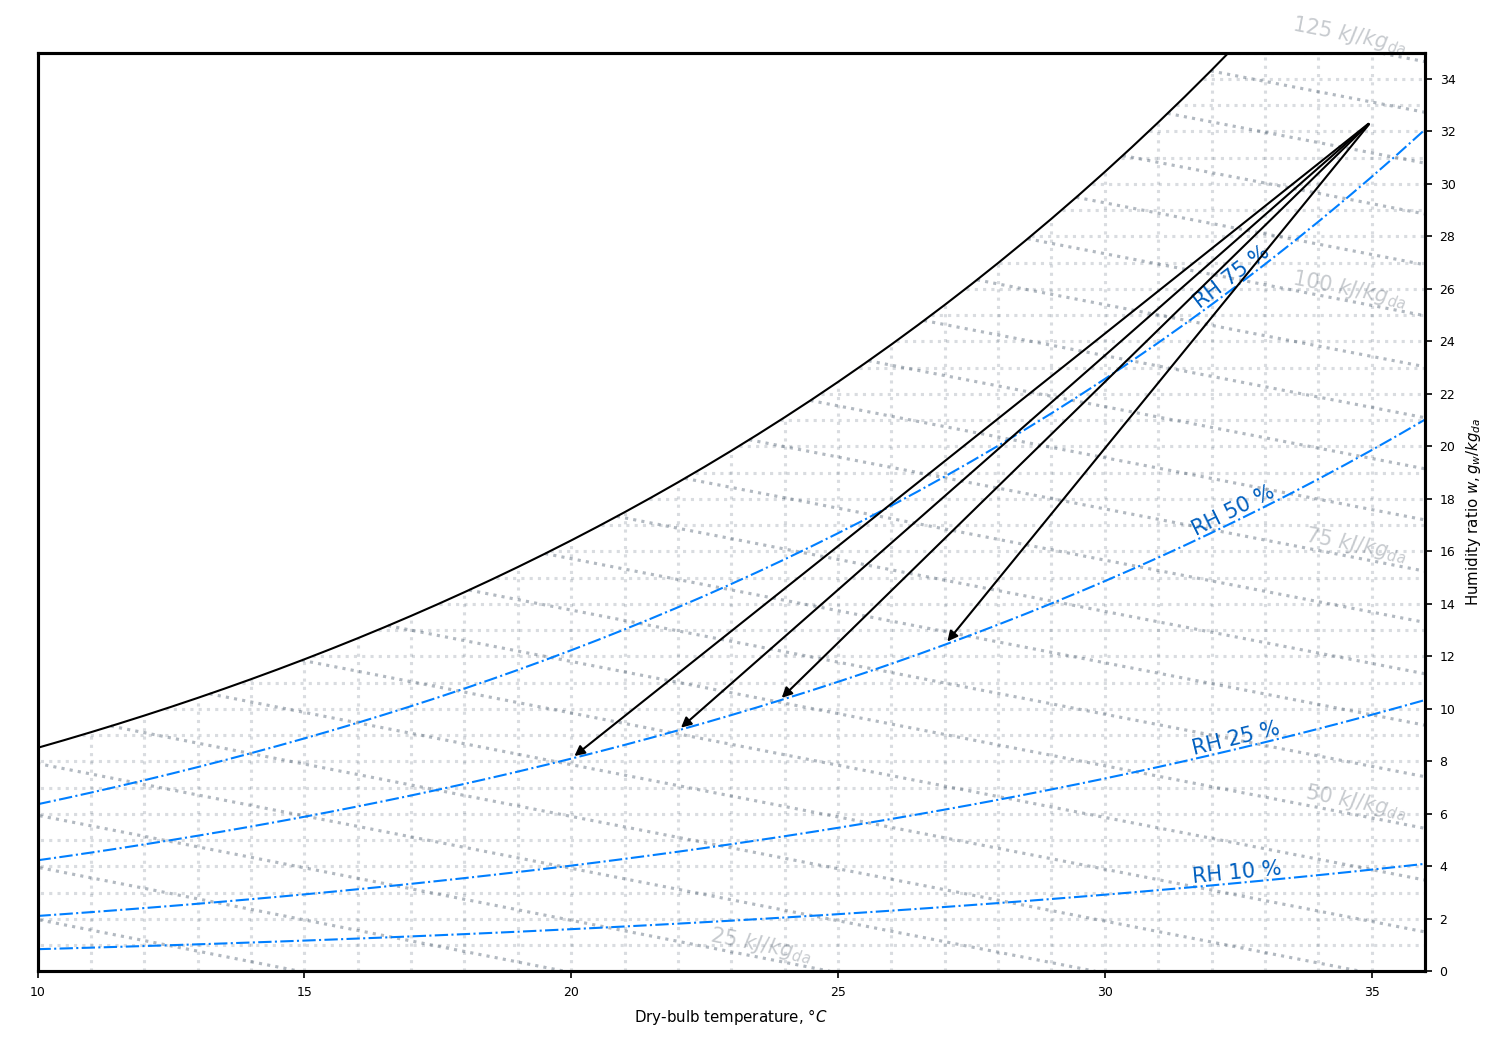
\includegraphics[width=\textwidth]{coolingcases.png}
    \caption{Example psychrometric processes under different set points for the cooling scenario.}\label{fg:cool}
    \end{figure}


    %This is how we calculate the changes in enthalpy against CDD. 
    We want to compare the impacts of having different set points specifically focusing on the differences in latent loads, which we are showing in the psychrometric process in the figure above. While maintaining the same level of desired RH, the changes in the energy demand is not fully reflected by the changes in dry bulb air temperature. We can explicitly compare the overall (latent and sensible) and sensible load by comparing the cooling degree days and the enthalpy degree days of identified set points for the cooling season and the outdoor temperature. 

    %Psychrometrically
    Psychrometrically speaking, this process is shown in Figure~\ref{fg:cool}, when air is cooled from the outdoor conditon with high dry-bulb temperature and relative humidity, eventuallly reaching the four different set points at the same desired level of RH: 50\%. The differences between the end-state enthalpy can be easily characterized by $\Delta h$ for the different set points and the outdoor temperature. We will compare this with the resulting hourly cooling degree days of each specific weather file. Following the definition of CDD by ASHRAE, we calculate the cooling degree days with Equation~\ref{eq:CDD}. Here, the cooling degree days for a defined reference temperature is $CDD_{t_{bal}}$ for a specific defined reference temperature $t_{bal}$. The rest of the parameters here are $n$ as the number of days over the desired period, and $\bar t_{o,i}$ as the daily average outdoor temperature ($\degree C$). For our purpose of the analysis, to analyze the different set points of the indoor air condition, we will use four different $t_{bal}$ values. The ASHRAE recommended set point range is 74$\degree F$to 80$\degree F$in the summer, while a typical radiant cooled space will use 75$\degree F$(24$\degree C$) air temperature with no greater than 50\% RH, which is the equivalent of a lower dew point temperature (approx. 12.2$\degree C$) to avoid condensation\cite{american_society_of_heating_2007_2007}.  The lowest will therefore be 18.3 $\degree C$ as suggested by ASHRAE for CDD calculation, with two extra data points as suggested by ASHRAE to be 23.3 $\degree C$ (74 $\degree F$) as well as 26.67 $\degree C$(or 80 $\degree F$, as recommended set point by ASHRAE) and up to 28 $\degree C$ (Sui \& Zhang, 2015) for the indoor air temperature in radiantly cooled environment. 

    \begin{equation}
    CDD_{t_{bal}} = \sum_{i=1}^n (\bar t_{o,i}-t_{bal})^{+}\label{eq:CDD}
    \end{equation} 

    To characterize the variations of the latent loads relating to only the enthalpy differences, the same set of dry bulb temperatures are used, while the enthalpy degree days are calculated similarly using Equation~\ref{eq:EDD}. Here, we characterize the total enthalpy differences between the state of the outdoor air ($\bar h_{o,i}$) that needs to be conditioned to a specific set point with enthalpy ($h_{bal}$). 

    \begin{equation}
    EDD = \sum^n_{i=1}(\bar h_{o,i}-h_{bal})\label{eq:EDD}
    \end{equation}

    To compare the sensible with the latent demand, the output from Equation~\ref{eq:CDD} (in Kelvin) needs to be compared with the output from Equation~\ref{eq:EDD} (kJ/kg of dry air). To achieve the same resulting unit, we will be multiplying the CDD values with the equation to calculate $c_p$ with Equation~\ref{eq:cp}, where the specific heat ($kJ/kg\cdot K$) can be calculated with a given  humidity ratio $w$. Multiplying CDD obtained through Equation~\ref{eq:CDD} with corresponding $c_p$, we may therefore obtain a specific enthalpy of dry air that is comparable to specific enthalpy of moist air obtained via Equatino~\ref{eq:EDD}/

    \begin{equation}
    c_p = 1.005 + 1.884 w \label{eq:cp}
    \end{equation}
    %This is actually the discussion of system sizing, which should go either to conclusion or discussion... Can expand to - what's going to happen when we simply change the set points in systems? 
    This calculation is aimed at emphasizing the amount of additional cooling needed when the feedback control variable is only dry bulb air temperature instead of both air and relative humidity. As is highlighted with green in the graph we generated, assuming the same amount of cooling capability but targeting only the dry bulb temperature instead of air mixture at different set points, the sizing  

\subsubsection{Heating Processes}
    %RH difference - map
    For the heating scenario, we will be operating under two stages of hypothesis. The first hypothesis we want to examine is there being no extra humidifier for the winter condition (i.e. no blue arrows in Figure~\ref{fg:heat}). The relative humidity would obviously be much higher when the set point is lower for radiant systems, and vice versa for the air-based system. Assuming a constant-humidity ratio heating process, we may therefore estimate the resulting RH for an average state during the heating season.  

    \begin{figure}[h!]
    \centering
    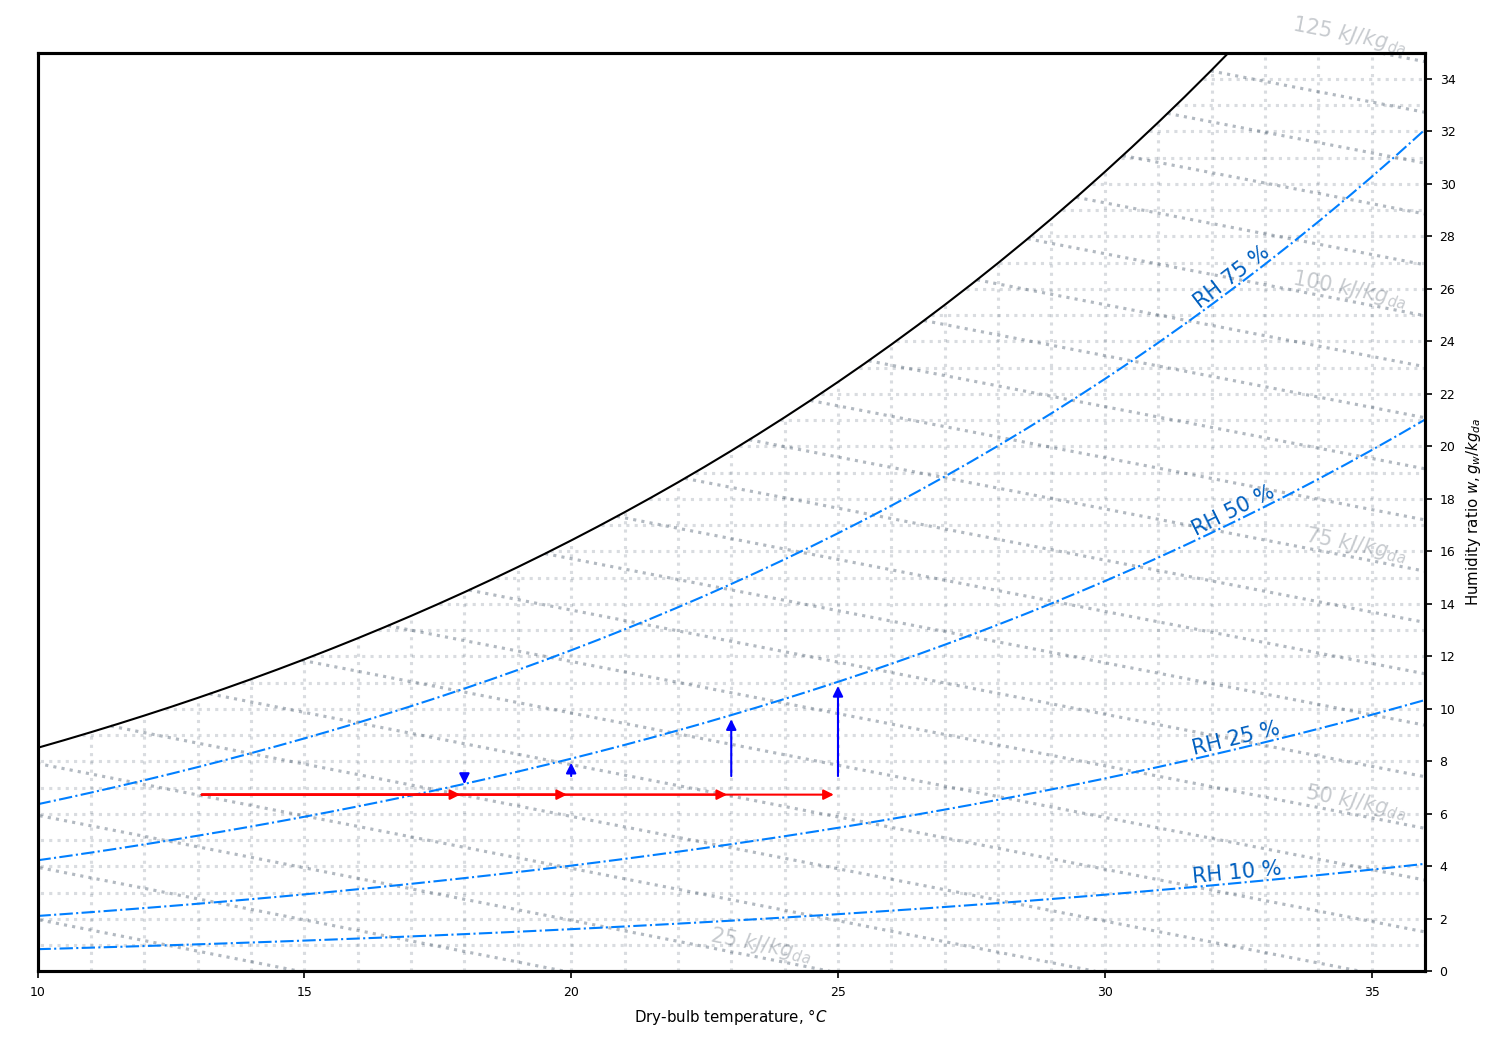
\includegraphics[width=\textwidth]{heatingcases.png}
    \caption{Example psychrometric processes under different set points for the heating scenario.}\label{fg:heat}
    \end{figure}

    Similar to the psychrometric process in the cooling case, we are expressing the heating of air in the psychrometric chart underneath. Since the majority of the heating is accomplished through furnaces and air conditioners, the outdoor air is assumed to go through a constant-humidity-ratio process as it is heated sensibly. Without additional humidifiers, the resulting RH could reach beneath 30\% (as indicated in the figure), and potentially lead risks of the occupants’ wellbeing. Even when considering additional humidifiers, the energy that needs to be added to the air can also be characterized as additional energy demands (as marked by the red arrows in illustration we created. %Check this paragraph

    It is, therefore, crucial to provide an estimation of the overall energy demand necessary to deliver air that is warm enough for all-air systems or radiant system, and additionally air that is moist enough to avoid strain on the respiratory system of the occupants. We believe it is crucial to highlight the energy savings in both the cooling and the heating condition when considering expanded set points. Using the psychrometric-driven approach, we are hoping to conduct both spatial and statistical analysis on the resulting RH and energy demand across continental US with the NOAA data we collected. %Check this paragraph

    %Energy difference - ratio of dry vs. latent.
    Beyond the first hypothesis, we would also like to assume an alternative scenario where humidifiers are used to ensure a satisfying humidity condition. This is expressed with the blue arrows in Figure~\ref{fg:heat}. With the added humidity into the air, the added latent load for all-air systems can be considered as the load that is not often characterized in the existing literature. Without specifying the systems that are used in this process and their respective efficiencies, analyzing only the requried latent load that needs to be added to the moist air through humidifier can help us understand the extra energy that is necessary when attempting to achieve desirable RH condition for the indoor environment across different set points. 

    %The RH difference will be compared with the mean value. The energy saving percentage will be compared with daily average? monthly average? heating season? 
    With respect to the set points, we will be assuming sensible heating only, where the outdoor air is heated up with the same humidity ratio. Following the indoor air temperature guideline recommended by ASHRAE, which is 68$\degree F$to 74$\degree F$(approximately 20 to 23$\degree C$) for winter, we will be using these temperatures as the base condition to be compared with. For the radiant scenario, since the radiant surfaces are often kept at a higher temperature, we will be setting the indoor air temperature slightly higher than that of the dew point temperature of assumed indoor air condition – which we assume to have a RH at 50\%. As was noted by Olesen in 2002, using radiant system means the air temperature can be kept at a lower temperature (2002). Examining more recent literature, we have therefore determined the lowest set point air temperature to be as low as 18 $\degree C$. 


